{
\begin{figure*}[th]
\begin{minipage}{\figWidthSix}
\begin{center}
\centerline{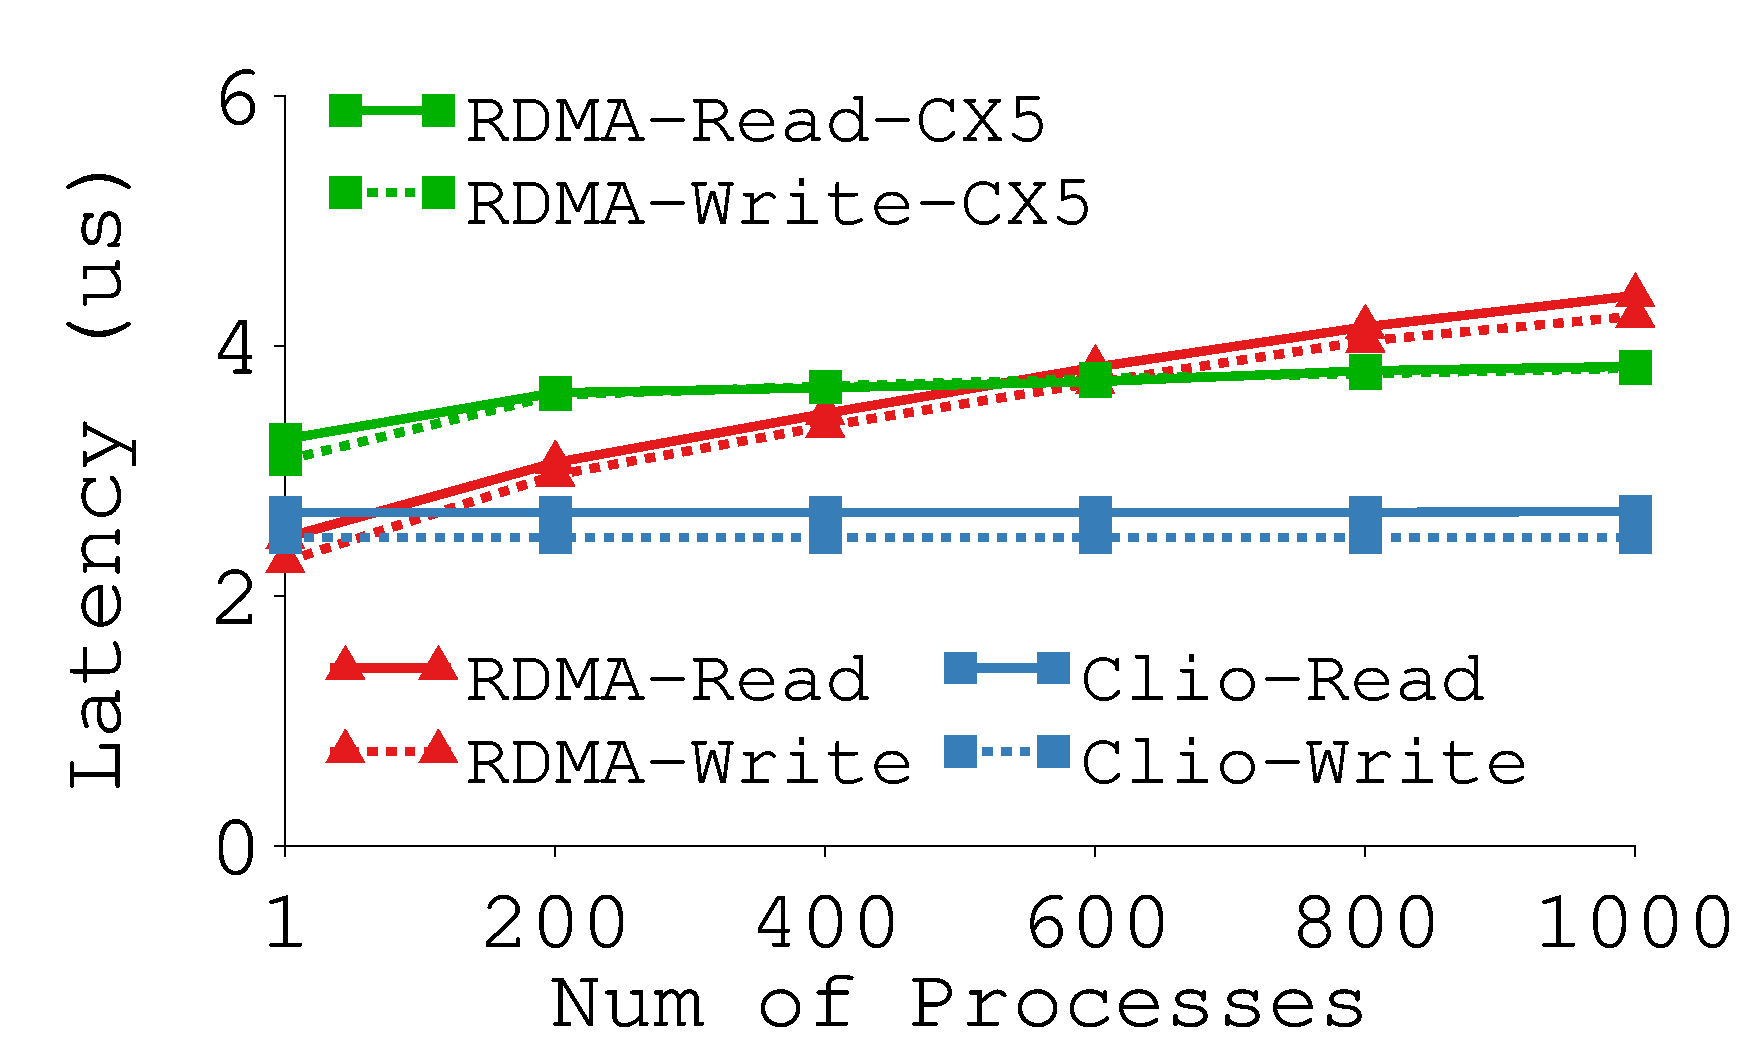
\includegraphics[width=\columnwidth]{Figures/g_plot_scalability_conn.pdf}}
\vspace{-0.1in}
\captionsetup{width=.9\columnwidth}
\mycaption{fig-conn}{Process (Connection) Scalability.}
{
}
\end{center}
\end{minipage}
%\begin{minipage}{0.01in}
%\hspace{0.01in}
%\end{minipage}
\begin{minipage}{\figWidthSix}
\begin{center}
\centerline{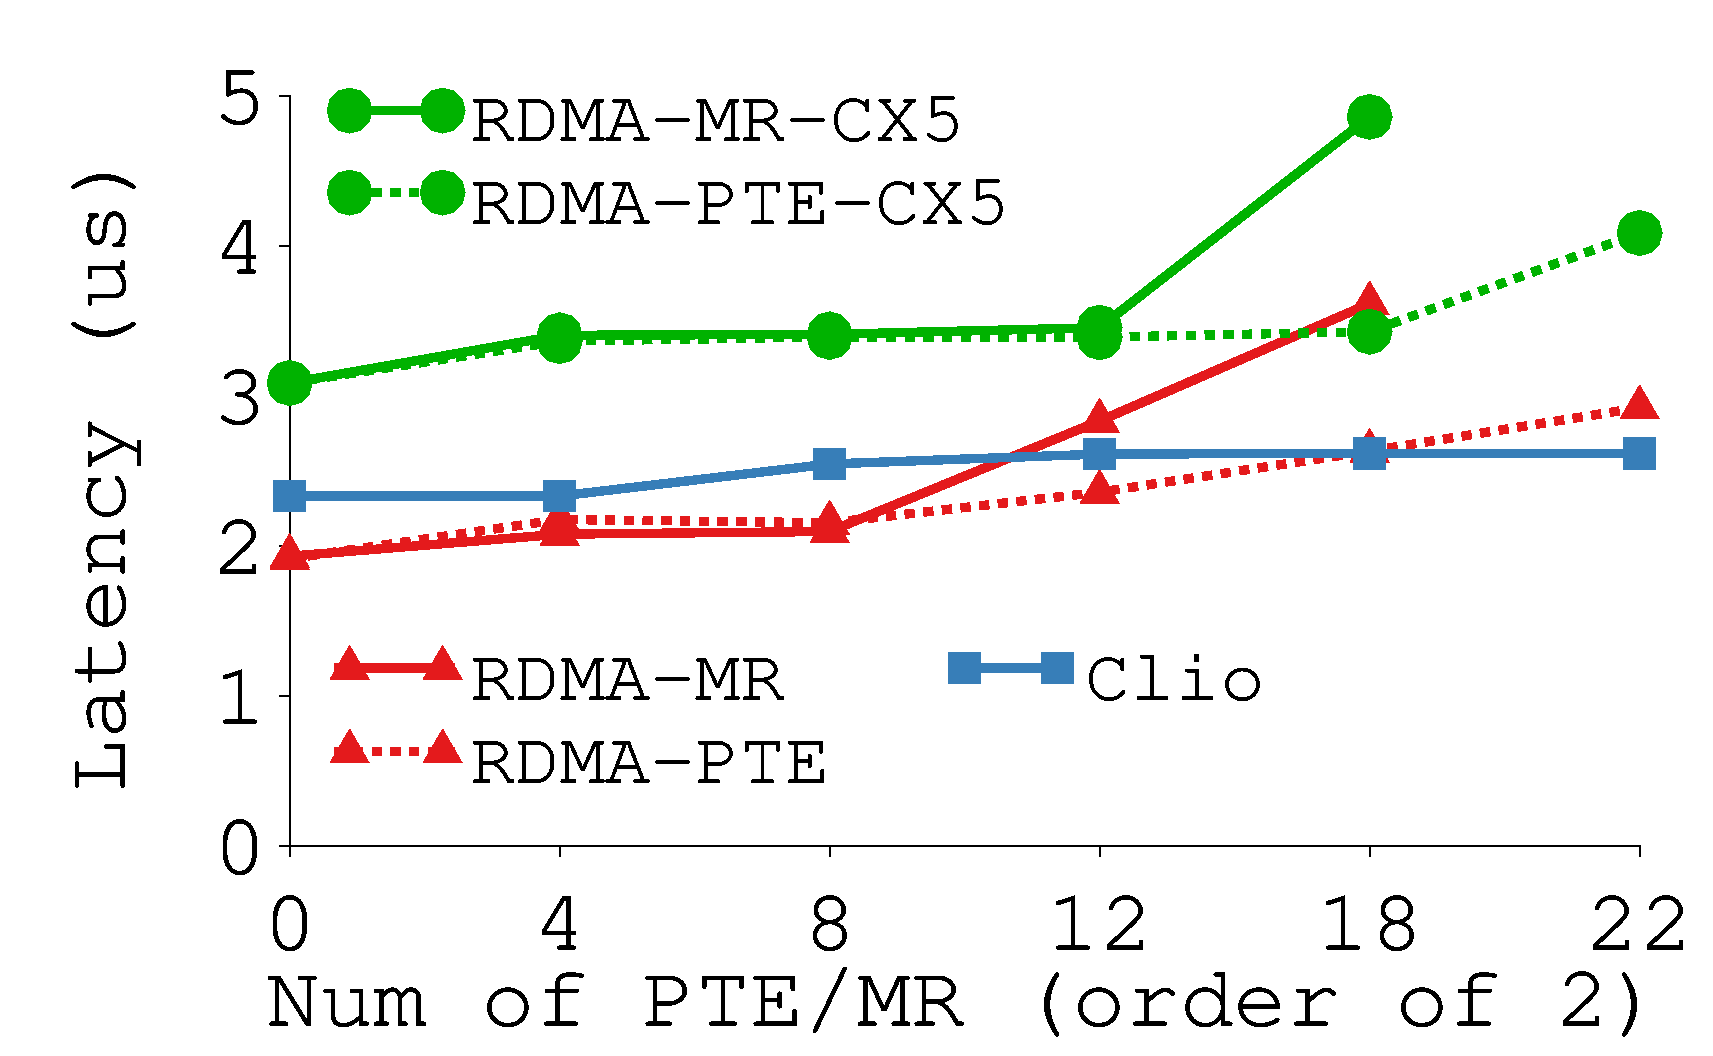
\includegraphics[width=\columnwidth]{Figures/g_plot_scalability_pte.pdf}}
\vspace{-0.1in}
\captionsetup{width=.9\columnwidth}
\mycaption{fig-pte-mr}{PTE and MR Scalability.}
{
RDMA fails beyond $2^{18}$ MRs. 
}
\end{center}
\end{minipage}
%\begin{minipage}{0.01in}
%\hspace{0.01in}
%\end{minipage}
\begin{minipage}{\figWidthSix}
\begin{center}
\centerline{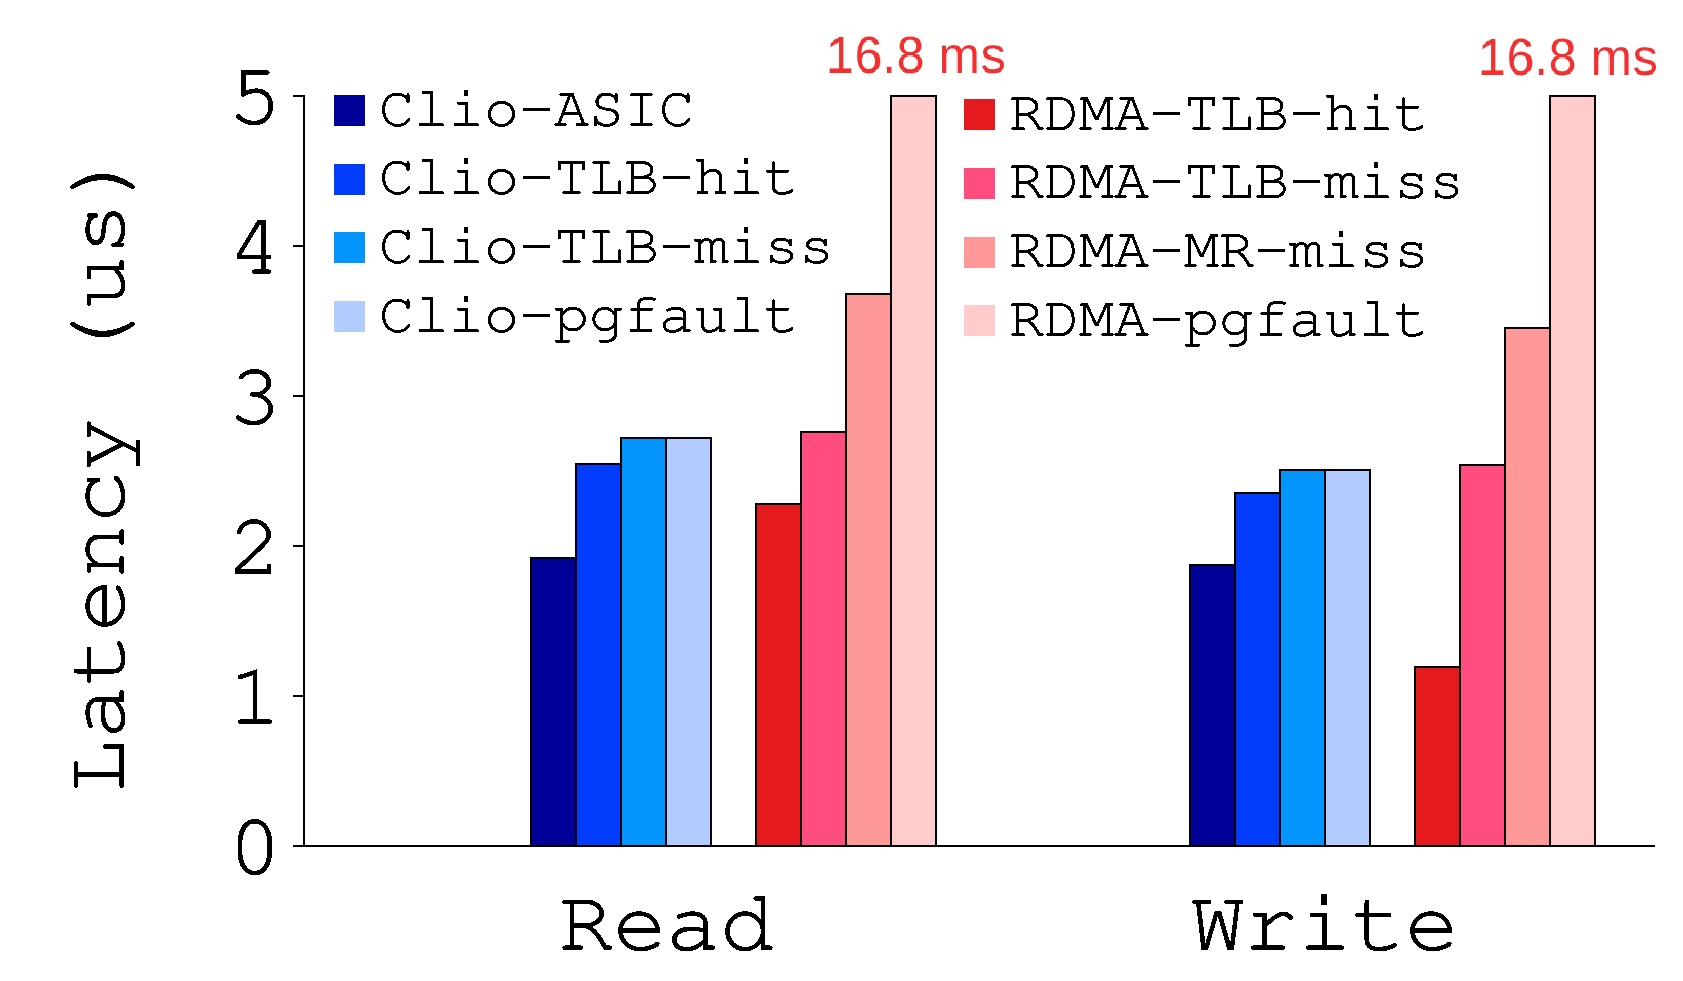
\includegraphics[width=\columnwidth]{Figures/g_plot_latency_comparison.pdf}}
\vspace{-0.1in}
\captionsetup{width=.9\columnwidth}
\mycaption{fig-miss-hit}{Comparison of TLB Miss and page fault.}
{
\sys-ASIC are projected values of TLB hit.
}
\end{center}
\end{minipage}
\begin{minipage}{\figWidthSix}
\begin{center}
\centerline{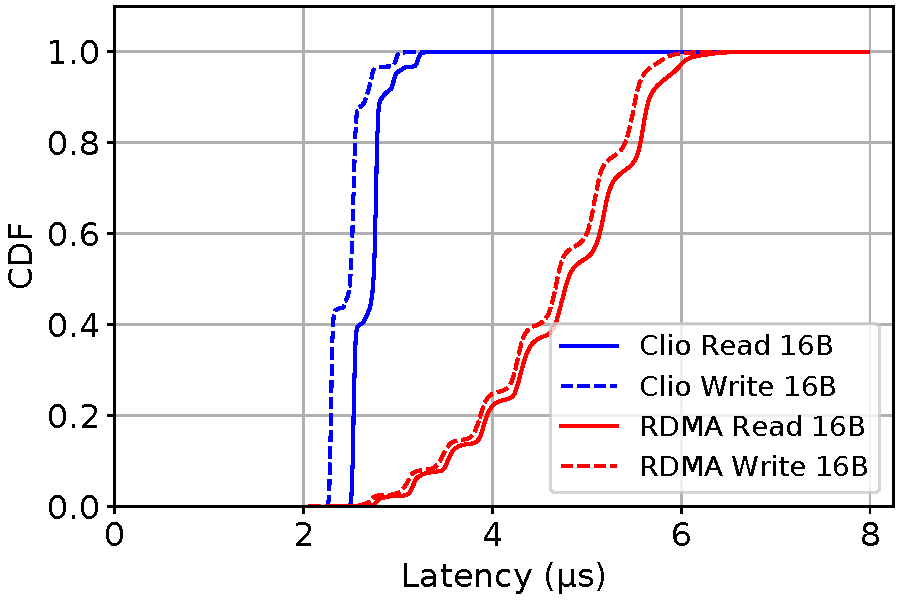
\includegraphics[width=\columnwidth]{Figures/clio_rdma_lat_cdf.pdf}}
\vspace{-0.1in}
\captionsetup{width=.9\columnwidth}
\mycaption{fig-tail-latency}{Latency CDF.}
{
}
\end{center}
\end{minipage}
\vspace{-0.1in}
\end{figure*}
}
